\documentclass[a4paper, 11 pt, onecolumn]{article}   % list options between brackets
\usepackage{graphicx, url}              % list packages between braces

\usepackage{enumerate}


\usepackage{fancyvrb}
\usepackage{amssymb,amsmath}
%\usepackage[top=3cm, bottom=3cm, left=3cm, right=3cm]{geometry}

\usepackage[utf8]{inputenc}
\usepackage[brazilian]{babel} 

% type user-defined commands here
\newcommand{\HRule}{\rule{\linewidth}{0.5mm}}
\newcommand{\barra}{\\[0.5cm]}

\hyphenation{ne-ga-ti-va}

\begin{document}

\title{Mineração de Dados - tp 3\\ KNN}   % type title between braces
\author{Thales Filizola Costa\\ \scriptsize{\textit{thalesfc@dcc.ufmg.br}}}         % type author(s) between braces
\date{\today \\ \HRule}    % type date between braces
\maketitle

\tableofcontents
\newpage

\section{INTRODUÇÃO}
Classificação é o problema de identificar para qual de um conjunto de categorias uma nova observação pertence, com base no treinamento utilizando dados com observações cuja a categoria é conhecida. 

O \textit{k-nearest neighbor}(KNN), um dos primeiros algoritmos de classificação criados, é de fácil entendimento. A ideia do algoritmo é classificar uma nova instância com base nas instâncias de treino. Sabendo os k vizinhos mais semelhantes somos capazes de predizer a classe da nova observação.

Este trabalho prático propõem a utilização do algoritmo de \textit{k-nearest neighbor}(KNN) para classificação de uma base de dados reais.

A seção \ref{basededados} retrata a base de dados utilizada neste trabalho, tendo como foco a análise de stemming e de retirada de stopwords e relacionando os mesmos com os efeitos na acurácia e na performance do algoritmo. 
Na seção \ref{valork} apresentamos uma discussão sobre a forma de escolha do parâmetro k. A seção \ref{sec:exp} retrata todos os experimentos executados.
 
\section{ALGORITMO DE \textit{K-NEAREST NEIGHBOR}}
\subsection{Descrição}
O algoritmo de \textit{k-nearest neighbor} é um método para classificação de objetos baseado na proximidade com exemplos de treinos em relação ao espaço de atributos. O funcionamento do algoritmo é apresentado abaixo:

\begin{enumerate}
  \item Dado um conjunto de trainamento da forma:$(x_1, y_1), (x_2, y_2) \cdots (x_n, y_n)$.
  \item Assumimos que $x_i= (fi_1, fi_2 \cdots fi_d)$ um vetor d dimencional de features, onde cada posição $t$ é a frequência do téssimo termo no ponto $i$.
  \item $y_i$ é a classe \{0, 1\} do ponto $i$.
  \item \underline{A tarefa:} determinar $y_{new}$ para todos os $x_{new}$.
\end{enumerate}
\paragraph{Algoritmo de kNN:}
\begin{enumerate}
\setcounter{enumi}{4}
 \item Encontre os k pontos mais próximos de $x_{new}$, usando uma métrica de distância, e.g. distância euclideana.
  \item Classifique $y_{new} = $ voto majoritário dentre os k pontos mais próximos. 
\end{enumerate}

Durante a execução do algoritmo de kNN, não é necessário estimar nenhum parâmetro, como por exemplo é feito no classificador Rocchio(centroides) ou no Naive Bayes(prioris e probabilidades condicionais). kNN simplesmente memoriza todos os exemplos de treino e compara o documento de teste com eles. Por essa razão, kNN é chamado de \textit{memory-based learnig} ou \textit{instance-based learning}. É sempre interessante ter a maior quantidade de instâncias de treino possíveis, entretanto, no kNN ter essas instâncias é um custo para o classificador. Maiores detalhes serão apresentados à seguir, quando falamos sobre a complexidade do algoritmo.


\subsection{Complexidade}
\label{complexidade}
Assim, o custo computacional do algoritmo de kNN para classificação de um simples ponto é $O(nd)$, onde $n$ é o número de pontos no treinamento e $d$ é a quantidade de dimensões do espaço de atributos, no nosso caso será o tamanho do vocabulário. O custo do algoritmo é esse pois para classificar um ponto, calculamos a distância desse ponto com todos os $n$ pontos de treinamento. O custo de calcular a distância entre dois pontos é $d$, logo o custo geral é $O(nd)$.


\section{MÁQUINA DE TESTE}
Todos as execuções e testes do programa implementado foram executadas na máquina:
\texttt{claro.grad.dcc.ufmg.br}

\section{BASE DE DADOS}
\label{basededados}
A base de dados utilizada consiste em \textit{reviews} de usuários para filmes. Para cada \textit{review} são fornecidos o comentário e a classificação do comentário, que pode ser positiva (1) ou negativa (0).

\subsection{Vocabulário}

Nessa subseção queremos determinar se, para os próximos experimentos, vamos utilizar ou não \textit{stemming} e se vamos retirar as \textit{stopwords}. 

A tabela \ref{tab:string} apresenta um sumários das diferentes configurações para tratamento de palavras. Nesses experimentos, o número de vizinhos utilizados foi dez (\texttt{k=10}) e a semelhança entre os pontos foi calculada utilizando a distância euclideana (\texttt{d=euclidean}).

\begin{table}[htp!]
\centering
\begin{tabular}{c c| c | c c}
 Stopwords   & Stem & Tamanho do & Acurácia & Tempo de  \\
 & & vocabulário & & execução$*$\\ \hline
 Não & Não & 31892 &0.6325\% &88.33 s\\
Não & Não & 31393 & 0.51\% &85.89 s \\
Não & \textbf{Sim} & 21562 &0.6675\% &63.81 s\\
\textbf{Sim} & \textbf{Sim} & 21127 &0.5175\% &62.59 s \\
\end{tabular}
\caption{Sumário das diferentes configurações para tratamento de strings.\label{tab:string} $*$ Média de 5 execuções}
\end{table}

De acordo com a tabela acima, podemos ver que o stemming reduziu bem a dimencionalidade dos dados (próximo de $\frac{1}{3}$) com melhoria na acurácia, por isso será adotado. Entretanto, a remoção das \textit{stopwords} não apresentou ganhos tão grandes de redução de dimencionalidade e levou a perda de acurácia, portanto essa prática não será adotada.

\subsection{Distribuição das classes}

A distribuição das classes determina a proporção de exemplos da partição que são das respectivas classes.
Conforme podemos ver pela figura \ref{fig:distclasses}, a partição de treino é desbalanceada em relação ao teste, visto que as proporções entre as classes são completamente diferentes ($\frac{1}{3}$ no treino e $1$ no teste).

\begin{figure}[htp!]
\hspace{-3.5cm}
 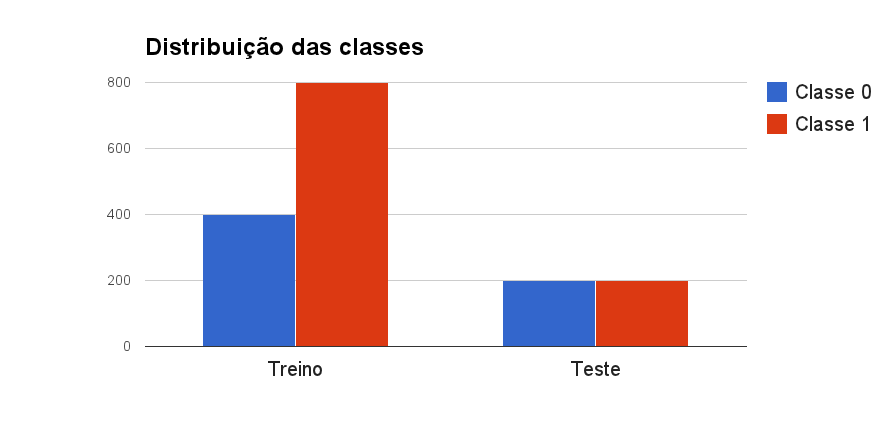
\includegraphics[scale=0.6]{imagens/chart_1.png}
  \caption{Distribuição das classes na base de dados. \label{fig:distclasses}}
\end{figure}

Tal distribuição atrapalha o algoritmo de classificação, pois com o dado treino existe uma probabilidade maior de classificar os pontos como sendo da classe 1.

\section{SELECIONANDO O VALOR DE K}
\label{valork}
O objetivo deste trabalho prático é simular um ambiente real de utilização do algoritmo de KNN. 
Como consequente não podemos utilizar a acurácia na partição de teste para escolhermos o melhor valor de $k$.

A solução é empregarmos a técnica de \textit{leave-one-out} nos dados de treino utilizando diferentes valores de $k$, com isso somos capazes de estimar qual o valor de $k$ que melhor se comporta para a base de dados.

\subsection{Leave-one-out}
A técnica de \textit{leave-one-out} é apresentada abaixo, tal técnica foi escolhida devido à sua resistência à variância e sua facilidade de computar.

\begin{enumerate}
 \item Para cada exemplo $e_i = (f, c)$ no treino:
 \begin{enumerate}
  \item Treino o classificador de KNN usando todos os pontos, menos $e_i$
  \item Teste a acurácia do classificador para $e_i$
 \end{enumerate}
  \item Repita o processo para todos os $i$ pontos
  \item Acurácia = média da acurácia de todos os pontos.
\end{enumerate}

\subsection{Resultados}

A configuração dos parâmetros utilizada nesses testes foi: uso de stemming sem a retirarada das stopwords.

Usando a técnica de \textit{leave-one-out}, testamos diversos valores de $k$ usando distância Euclideana e de Jaccard. 

As tabelas \ref{tab:leave} e \ref{tab:leave_jaccard} apresentam respectivamente os resultados obtidos para as distâncias  Euclideana e Jaccard. Dos diversos valores de k testados reportamos: no campo de treino (leave-one-out), a acurácia e o tempo de execução; no campo de teste, somente a acurácia. A figura \ref{fig:leave} apresenta um resumo das acurácias na partição de treino.

\begin{table}[htp!]
\centering
 \begin{tabular}{l|c c|c}
  \textbf{}& \multicolumn{2}{|c|}{\textbf{TREINO}} & \textbf{TESTE}\\ \hline
  \textbf{Valor de k} &\textbf{Acurácia(\%)}&\textbf{Tempo de execução (s)} & \textbf{Acurácia (\%)}\\ \hline
    k=1 & 0.6258  & 281.48  & 0.615 \\
    k=3 & 0.6433  & 282.09  & 0.6075\\
    k=5 & 0.6775  & 280.63  & 0.6425\\
    k=7 & 0.68  & 280.36  & 0.65\\
    k=9 & 0.6958  &285.94  & 0.63\\
    k=15 & 0.68  & 284.73  &  0.6275\\
    \textbf{k=30} & \textbf{0.6925}  & \textbf{285.96} & \textbf{0.5925 }\\
    k=40 &  0.69 & 282.77  & 0.5725\\
    k=50 &  0.695 & 285.1 & 0.5725 \\
    k=100 & 0.6825  & 300.13  &0.5225\\
 \end{tabular}
  \caption{\label{tab:leave} \textit{Leave-one-out} na partição de treino usando distância Euclideana.}
\end{table}

Ainda analisando as tabelas \ref{tab:leave} e \ref{tab:leave_jaccard}, usando os valores de acurácia gerado pelo treino, $k=30$ é o melhor valor, entretanto, analisando os valores gerados pela acurácia no teste, vemos que o valor de $k=7$ obtem a melhor acurácia. A diferença no melhor valor de k para o traino e o teste é explicado pelo fato da distribuição de classes ser bem diferente.

\begin{table}[htp!]
\centering
 \begin{tabular}{l|c c | c}
  \textbf{}& \multicolumn{2}{|c|}{\textbf{TREINO}} & \textbf{TESTE}\\ \hline
  \textbf{Valor de k} &\textbf{Acurácia(\%)}&\textbf{Tempo de execução (s)} & \textbf{Acurácia (\%)}\\ \hline
    k=1 & 0.653  & 759.91 & 0.605\\
    k=3 & 0.683   & 753.78 & 0.6525\\
    k=5 & 0.7075  & 751.28 & 0.65\\
    k=7 & 0.7108  & 770.02 & 0.6875\\
    k=9 & 0.7108  & 759.36 &0.6775 \\
    k=15 & 0.7325   & 760.58 & 0.6625 \\
    k=20 & 0.7408  & 762.81 & 0.665 \\
    \textbf{k=30 }& \textbf{0.7433}  & \textbf{757.56} & \textbf{0.64}\\
    k=40 & 0.7441  & 763.13 & 0.6375\\
    k=50 & 0.7325  & 754.4 &0.6225\\
    k=100 & 0.7016   & 767.52 & 0.57\\
 \end{tabular}
  \caption{\label{tab:leave_jaccard} \textit{Leave-one-out} na partição de treino usando distância Jaccard.}
\end{table}

\begin{figure}
 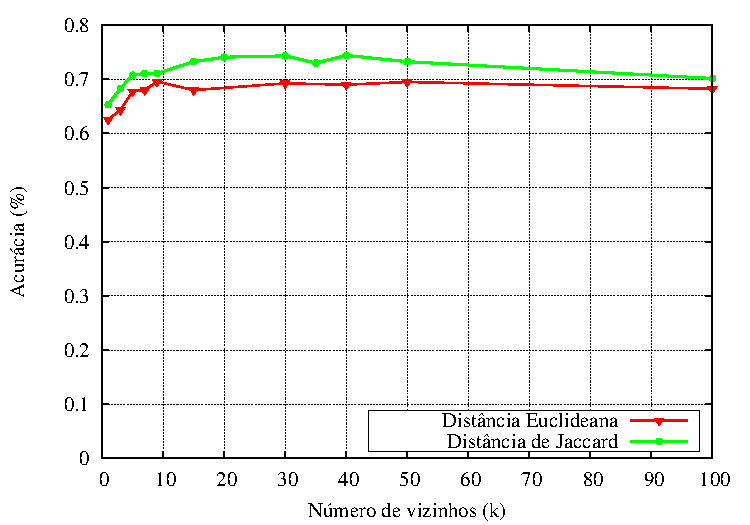
\includegraphics{imagens/leave_out.pdf}
 \caption{\label{fig:leave} Gráfico com resumo da técnica leave one out.}
\end{figure}

\pagebreak

\section{EXPERIMENTOS}
\label{sec:exp}

\subsection{Métricas de Distâncias}
Nessa seção vamos testar a qualidade de diversas métricas de distância no calculo do knn.
A configuração dos parâmetros utilizada nesses testes foi: uso de stemming, sem a retirarada das stopwords e \texttt{k=7}.

\begin{figure}
 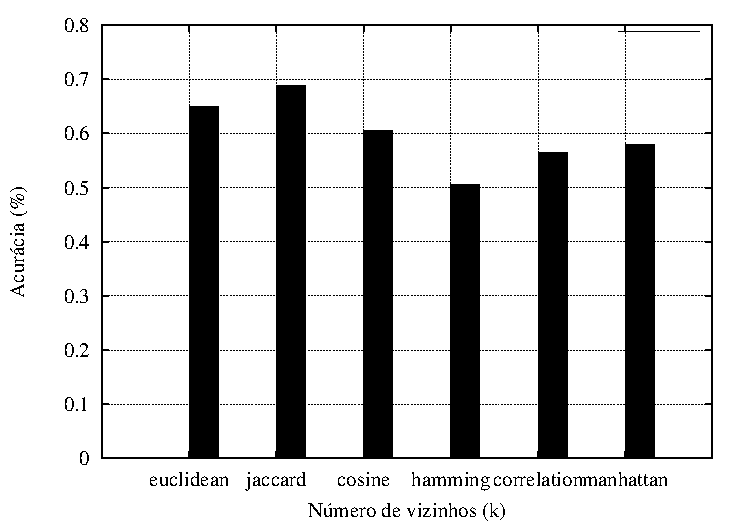
\includegraphics{imagens/distance.pdf}
 \caption{\label{fig:distance} Gráfico com resultado final para diversas distâncias.}
\end{figure}

Podemos ver pela figura \ref{fig:distance} que os melhores resultados foram obtidos pelas distâncias Euclideanas e de Jaccard.

\pagebreak

\subsection{Variaçaõ no Tamanho de Entrada}
Nessa seção vamos testar a estabilidade do algoritmo de knn com a variação no tamanho de entrada.
A configuração dos parâmetros utilizada nesses testes foi: uso de stemming, sem a retirarada das stopwords, \texttt{k=7} e distância de jaccard.

A metodologia adota será utilizar i\% do treino para classificar toda a base de teste. Sendo que o valor de $i$ vai de 10\% até 100\%.

Podemos ver pelas figuras \ref{fig:entrada} e \ref{fig:entrada2} que tanto o tempo de execução como a acurácia dos classificadores aumenta linearmente com a quantidade de dados no treino. Essas observações são importantes porque: (i) comprovam que complexidade do algoritmo é linear com o número de treinamento; (ii) mostram que a acurácia do algoritmo é proporcional ao número de treinamento. Logo se um pesquisador quiser melhorar a acurácia do classificador, uma maneira é investir em mais exemplos; e (iii) demonstra que existe um trade-off entre aumentar o número de treino para melhorar a acurácia, mas sofrer com o aumento do tempo de execução do algoritmo.

\begin{figure}
 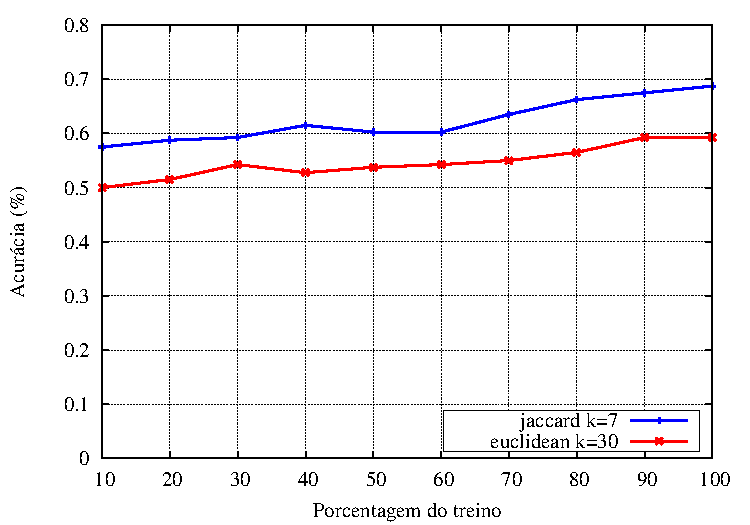
\includegraphics{imagens/entrada.pdf}
 \caption{\label{fig:entrada} Acurácia dos classificadores para diferentes porcentagens de treino.}
\end{figure}

\begin{figure}
 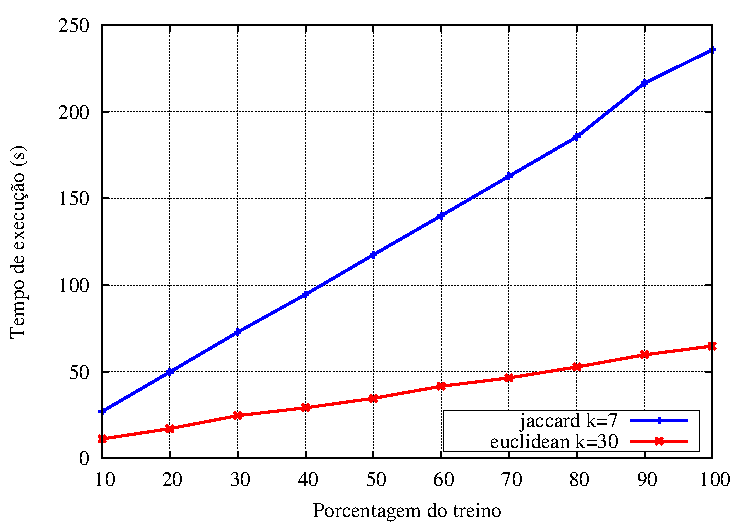
\includegraphics{imagens/entrada2.pdf}
 \caption{\label{fig:entrada2} Tempo de execução dos classificadores para diferentes porcentagens de treino.}
\end{figure}

\pagebreak

\section{CONCLUSÃO}
A realização deste trabalho prático permitiu algumas conclusões sobre o algoritmo de knn.
\begin{enumerate}
 \item A distribuição das classses no treino é muito diferente da distribuição das mesmas no teste. Essa diferença nas distribuições tem muita probabilidade de acontecer na implementação de sistemas reais, ao longo desse relatório foi demostrado que esse efeito pode afetar a acurácia do classificador e deve ser levado em consideração em implementações.
\item O efeito do stemming na base de dados obteve uma surpreendente melhoria na acurácia, o que sugere que a substituição de sinônimos possa ser explorada como trabalhos futuros para uma melhora ainda mais significativa dos resultados.
\item A técnica de \textit{leave-one-out} foi executada usando as distâncias Euclideana e de Jaccard. Tal técnica mostrou estabilidade ao obter melhores valores de k bem similares nas duas métricas. Entretando, devido à distribuição das classes ser bem diferente no treino/teste, os valores de acurácia obtidos (através do leave-one-out) não foram compatíveis com os valores obtidos no teste.

\item Os experimentos feitos com a técnica de leave-one-out mostram que o valor de $k$ não afeta o tempo de execução do algoritmo. Além disso, os resultados obtidos com a variação no tamanho de entrada mostram que o algoritmo tem custo computacional linearmente proporcional ao tamanho do treino. Esses dois resultados comprovam a complexidade do algoritmo derivada na seção \ref{complexidade}.

\end{enumerate}

%%  --------------- end of document
\nocite{meira}
\nocite{urlMetrics}

\bibliographystyle{plain}
\bibliography{reuniao}

\end{document}
